\documentclass[conference]{IEEEtran}
\usepackage{times}

% numbers option provides compact numerical references in the text. 
\usepackage[numbers]{natbib}
\usepackage{multicol}
\usepackage[bookmarks=true]{hyperref}
\usepackage{graphicx}
\usepackage{amsmath,amsfonts,amssymb}
\usepackage{hyperref}

\graphicspath{ {./graphics/} }

\pdfinfo{
   /Author (Mingyo Seo)
   /Title  (Robots: Our new overlords)
   /CreationDate (D:20101201120000)
   /Subject (Robots)
   /Keywords (Robots;Overlords)
}

\begin{document}

% paper title
\title{CS391L HW2: Independent Component Analysis}

% You will get a Paper-ID when submitting a pdf file to the conference system
\author{Mingyo Seo}

\author{\authorblockN{Mingyo Seo}
\authorblockA{
UT EID: ms84662\\
Email: mingyo@utexas.edu}}



\maketitle

\IEEEpeerreviewmaketitle

\begin{abstract}
In this assignment, an overview of Independent Component Analysis (ICA) is presented and is applied to separate a mixture of sounds. We used a dataset of 5 different sources and mixed signals to generate multiple simulated "microphone" sounds. The ICA method was applied with Maximum Likelihood Estimation (MLE) and gradient descent to extract the individual sounds, and the separating performance was evaluated.
\end{abstract}

\section{Introduction} % Introduce your problem and the overall plan for approaching your problem

The problem of separating a certain signal from a mixture of multiple signals can be applied to many areas. The simplest example of this is the cocktail party problem, where we have recordings from different microphones of the same mixture of conversations.
In this paper, in particular, we implemented an ICA to seperate voices from the mixture of conversations. 
We also studied the effects of parameters on the model's performance. The answers to the HW2 questions are included in the following sections.\begin{itemize}
\item Fig. \ref{fig:signal}: Visualization of base, mixed, recovered signals
\item Fig. \ref{fig:basic_test}, \ref{fig:basic_abs_test}, \ref{fig:batch_abs_test}, \ref{fig:eta_abs_test}, \ref{fig:sample_abs_test}: Correlation between source and recovered signals
\end{itemize}



\section{Method}
\label{sec:method}

\subsection{Mixing matrix}

In this assignment, a test data set $U$ containing $5$ sound sources and $t$ number of samples is given. We aim to mix $n$ sources from the given sounds to generate a pseudo microphone output $X$ of $m$ recordings where $m\geq n$. To do this, we introduce a mixing matrix $A$, as
\begin{equation}
    X = AU
\end{equation}
Here, $X$ is a $m \times t$ matrix of the mixed sound signals.


\subsection{Independent Component Analysis}

Contrary to Principal Component Analysis which finds the primary features in the given dataset, the ICA method decomposes a mixture of signals into its individual sources. 

The goal of the ICA method is to find the un-mixing $n \times m$ matrix $W$, as
\begin{equation}
    WA = I.
\end{equation}
This yields of restoring the orignial signal $U$, as
\begin{equation}
    U = WX.
\end{equation}
We use the maximum likelihood estimate to find $\hat{W}$, an estimate of $W$, and the gradient descent to approximate it. These methods are described in the following subsections.


\subsection{Maximum Likelihood Estimation}

Computing the unmixing matrix $W$ can be implemented by the singular value decomposition (SVD), which requires the computation of the Eigenvalues of $XX^T$, which slows down the speed at a large number of sample recordings $m$.
On the other hand, the Maximum Likelihood Estimation (MLE) method can be used to find the optimal unmixing $W$ that maximizes optimization criteria $L(W)$ to match the mixed signals $X$.

As a criteria  $L(W)$, the following likelihood is used.
\begin{equation}
\begin{aligned}
     p_x(X) &= p_u(U)\cdot|W| \\
    & = \prod_{i=1}p_i(u_i)|W|    
\end{aligned}
\end{equation}
Here, $p_u(U)$ is the probability density function (PDF) of the source signals, and $p_i(u_i)$ is the probability density of the $i_{th}$ source component.
Then, we can rewrite $p_x(X)$ in terms of $t$ mixed samples $x_j: X= \left[x_1, ... , x_t \right]$ and use it as the optimization criteria, as
\begin{equation}
\begin{aligned}
    L(W) = p_x(X) =  \prod_{j=1}^t\prod_{i=1}^np_i(w_i^Tx_j)|W|.
    \label{eq:likelihood def}
\end{aligned}
\end{equation}

From the property that PDF is always positive, we can take log of $L(W)$ to changes the product terms in $W$ into summation terms, as
\begin{equation}
\begin{aligned}
    \ln{(L(W))} 
     &= \sum_{j=1}^t\sum_{i=1}^n\ln{(p_i(w_i^Tx_j)|W|)}\\
     &= \sum_{j=1}^t\sum_{i=1}^n\ln{(p_i(w_i^Tx_j)} + \sum_{i=1}^n\ln(|W|)\\
     &= \sum_{j=1}^t\sum_{i=1}^n\ln{(p_i(w_i^Tx_j)} + t\ln{(|W|)},
     \label{eq:simplified loglike}
\end{aligned}
\end{equation}
which is called {\it log likelihood}. Here, we can maximize $L(W)$ by maximizing the log likelihood. Further, we can rewrite Equation \ref{eq:simplified loglike}, as
\begin{equation}
    \frac{1}{t}\ln{(L(W))} = E\left[\sum_{i=1}^n\ln{(p_i(w_i^Tx_j))}\right] + \ln{(|W|)}.
    \label{eq:log-like-Exp}
\end{equation}
Let $g(X)$ be the cumulative density function (CDF) of the PDF $p_x(X)$.
The CDF $g(X)$ is the integral of $p_x(X)$, so $p(X)$ is the derivative of $g(X)$, as
\begin{equation}
    \frac{1}{t}\ln{(L(W))} = E\left[\ln{(g'(WX)}\right] + \ln{(|W|)}.
    \label{eq:log-like-Exp-cdf} 
\end{equation}


\subsection{Gradient descent}

The gradient descent method is an iterative algorithm to find a function's minimum or maximum points. If the convex function is convex, the gradient descent converges to the global extremums. Otherwise, it converges to the local extremums. Proving the convexity of the log likelihood $L(W)$ is beyond the scope of this report, so it is not described in this report.

Gradient descent starts at an initial point $\hat{W}_0$ and updates it by moving to next points recursively along the gradient computed at previous points. To formulate the gradient descent method in terms of $W$, the estimate $\hat{W}_{k}$ of the $W$ matrix after the $k^{th}$ iteration is given, as 
\begin{equation}
\begin{aligned}
    \hat{W}_{k+1} &= \hat{W}_k + \eta\cdot\left(\frac{1}{t}\frac{\partial}{\partial W}\ln(L(W))\right)_{W=\hat{W}_k}\\
     &= \hat{W}_k + \eta\cdot\Delta W,
\end{aligned}
\end{equation}
where $\eta$ is the {\it learning rate} of the gradient descent.
Here, the initial point $\hat{W}_0$ is given randomly, and $\eta$ should be adjusted to achieve convergence.

From Equation \ref{eq:log-like-Exp}, we can compute the gradient of $L(W)$, as
\begin{equation}
\begin{aligned}
    \frac{1}{t}\frac{\partial}{\partial W}\ln(L(W)) 
    &= E\left[\frac{\partial}{\partial W}(\ln{(g'(WX)})X^T\right] + \frac{\partial}{\partial W}\ln{(|W|)} \\
    &= E\left[\frac{\partial}{\partial W}(\ln{(g'(WX)})X^T\right] + \left[W^T\right]^{-1}.
\end{aligned}
\end{equation}
Here, the gradient term contains $\left[W^T\right]^{-1}$ which requires expensive computation for the inverse operation. 
Thus, we process the interation by multiplying it with $W^TW$, which preservers the convergence to the optimum, and avoids the inverse operation, as
\begin{equation}
\begin{aligned}
    \Delta W
    &= \frac{1}{t}\frac{\partial}{\partial W}\ln(L(W)) W^T \\
    &= E\left[\frac{\partial}{\partial W}(\ln{(g'(WX)})X^T\right] W^TW + \left[W^T\right]^{-1} W^TW \\
    &= \left(E\left[\left(\frac{\partial}{\partial W}(\ln{(g'(WX)})\right)(WX)^T\right] W + W\right)_{W=\hat{W}_k}.
    \label{eq:delta W simplified}
\end{aligned}
\end{equation}
The above formulation does not affect the optimality of Equation \ref{eq:simplified loglike}. The description for this is omitted for brevity of this report, and we encourage referring to the class notes.

To facilitate the gradient descent algorithm, we need to choose a globally differentiable CDF. In particular, we used the following CDF,
\begin{equation}
    g(WX) = \frac{1}{1+e^{-WX}}.
\end{equation}
It is differentiable for all $WX$ and is bounded in $\left[0,1 \right]$. The derivative of $g$ is given as
\begin{equation}
\label{eq:deriv}
    g'(WX) = g(WX)(1-g(WX)).
\end{equation}
Inserting Equation \ref{eq:deriv} into Equation \ref{eq:delta W simplified} yields
\begin{equation}
    \Delta W = \left(\left(E\left[(1-2g(WX))(WX)^T\right] + I \right)W\right)_{W=\hat{W}_k}.
\end{equation}

To summarize the processes described above, the algorithm is implemented, as
\begin{enumerate}
    \item Start with an intial point $\hat{W}_0$.  
    \item Compute matrix $Z_k = g(\hat{W}_kX)$
    \item Compute $\Delta W = \left(E\left[(1-2Z_k)(\hat{W}_kX)^T\right] + I \right)\hat{W}_k$.
    \item Update the estimation as $\hat{W}_{k+1} = \hat{W}_k + \eta\cdot\Delta W$
    \item Return to Step 2 and repeat the processes until it reaches the maximum iteration.
\end{enumerate}


\section{Results} % Describe the methods you intend to apply to solve the given problem

The ICA implementation of using MLE and gradient descent described in Section \ref{sec:method} is implemented under the environment of python scripts (3.8.5) and numpy (1.17.5). The model is trained and evaluated by the sound dataset from the class website \cite{cs391}. We used random mixes of $n=3$ source signals from the dataset and initialized $W_0$ to be random matrices where each entry in $[0, 1]$.


\subsection{Signal restoration}

In the assignment, the performance of the model is evaluated by correlation between original signals and recovered signals. We paired a restored signal with the orignal signal that has the largest magnitude of correlation. In the experiment, we used $n=3$, $m=3$, $\eta=0.01$, $t=16$ and the maximum interation $k_{\text{max}} = 5000$.

The source signals, the mixed signals, and the restored signals after $k_{\text{max}}$ are presented in Fig. \ref{fig:signal}.
The plot of correlation between the source signals and the restored signals is presented in Fig. \ref{fig:basic_test}.

Due to the semi-symmetric nature of waves, the largest correlation of Signal \#3 became negative, which implies that the extracted signal has the opposite phase of the original source signals. We use the plot of absolute correlation as Fig. \ref{fig:basic_abs_test} and find that correlation increase as an iteration number increases. For readability, we use absolute correlation for analyzing the effectiveness of the model in the following subchapters. Also, we can find that each source signal matches with the paired signals, which implies the ICA model successfully extracts original signals from mixed signals.

\begin{figure}[!t]
	\centering
	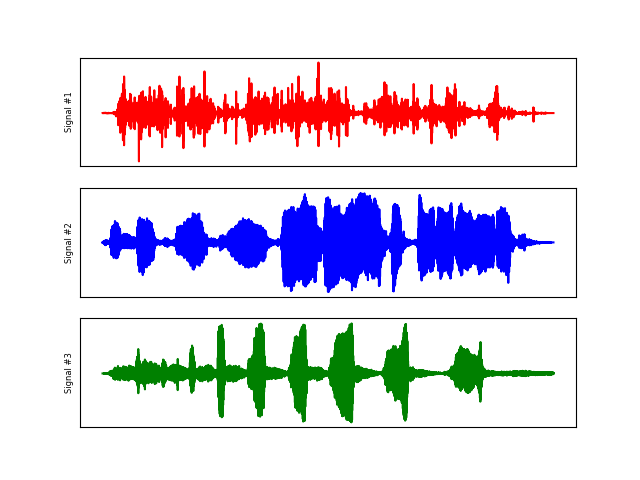
\includegraphics[width=3.6in]{original.png}	
	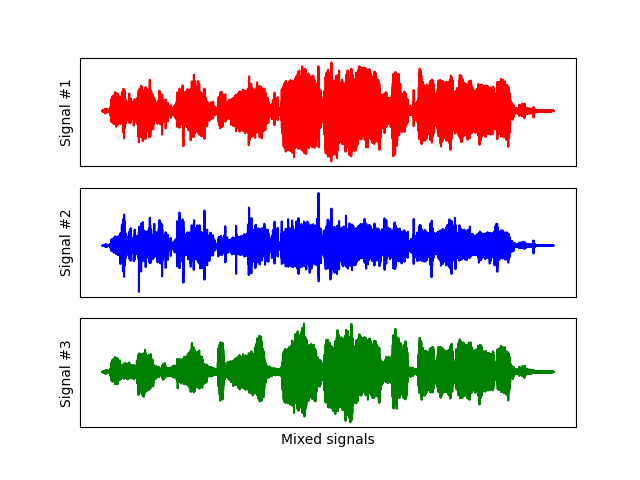
\includegraphics[width=3.6in]{mixed.png}	
	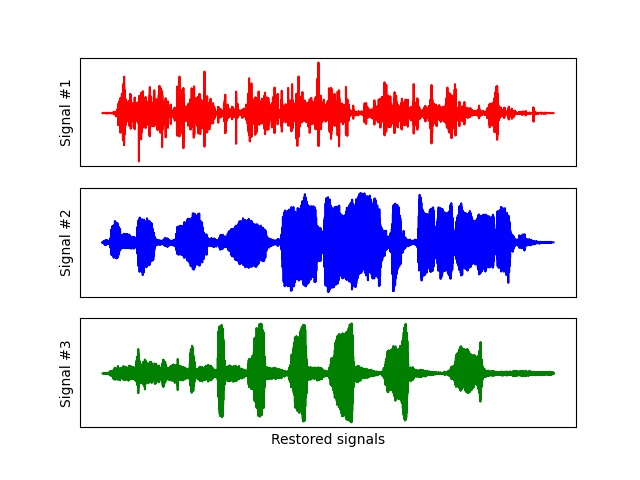
\includegraphics[width=3.6in]{restored.png}	
	\caption{Visualization of the signals: (upper) orignal signals, (middle) mixed signals, and (bottom) restored signals}
	\label{fig:signal}
\end{figure}

\begin{figure}[!t]
	\centering
	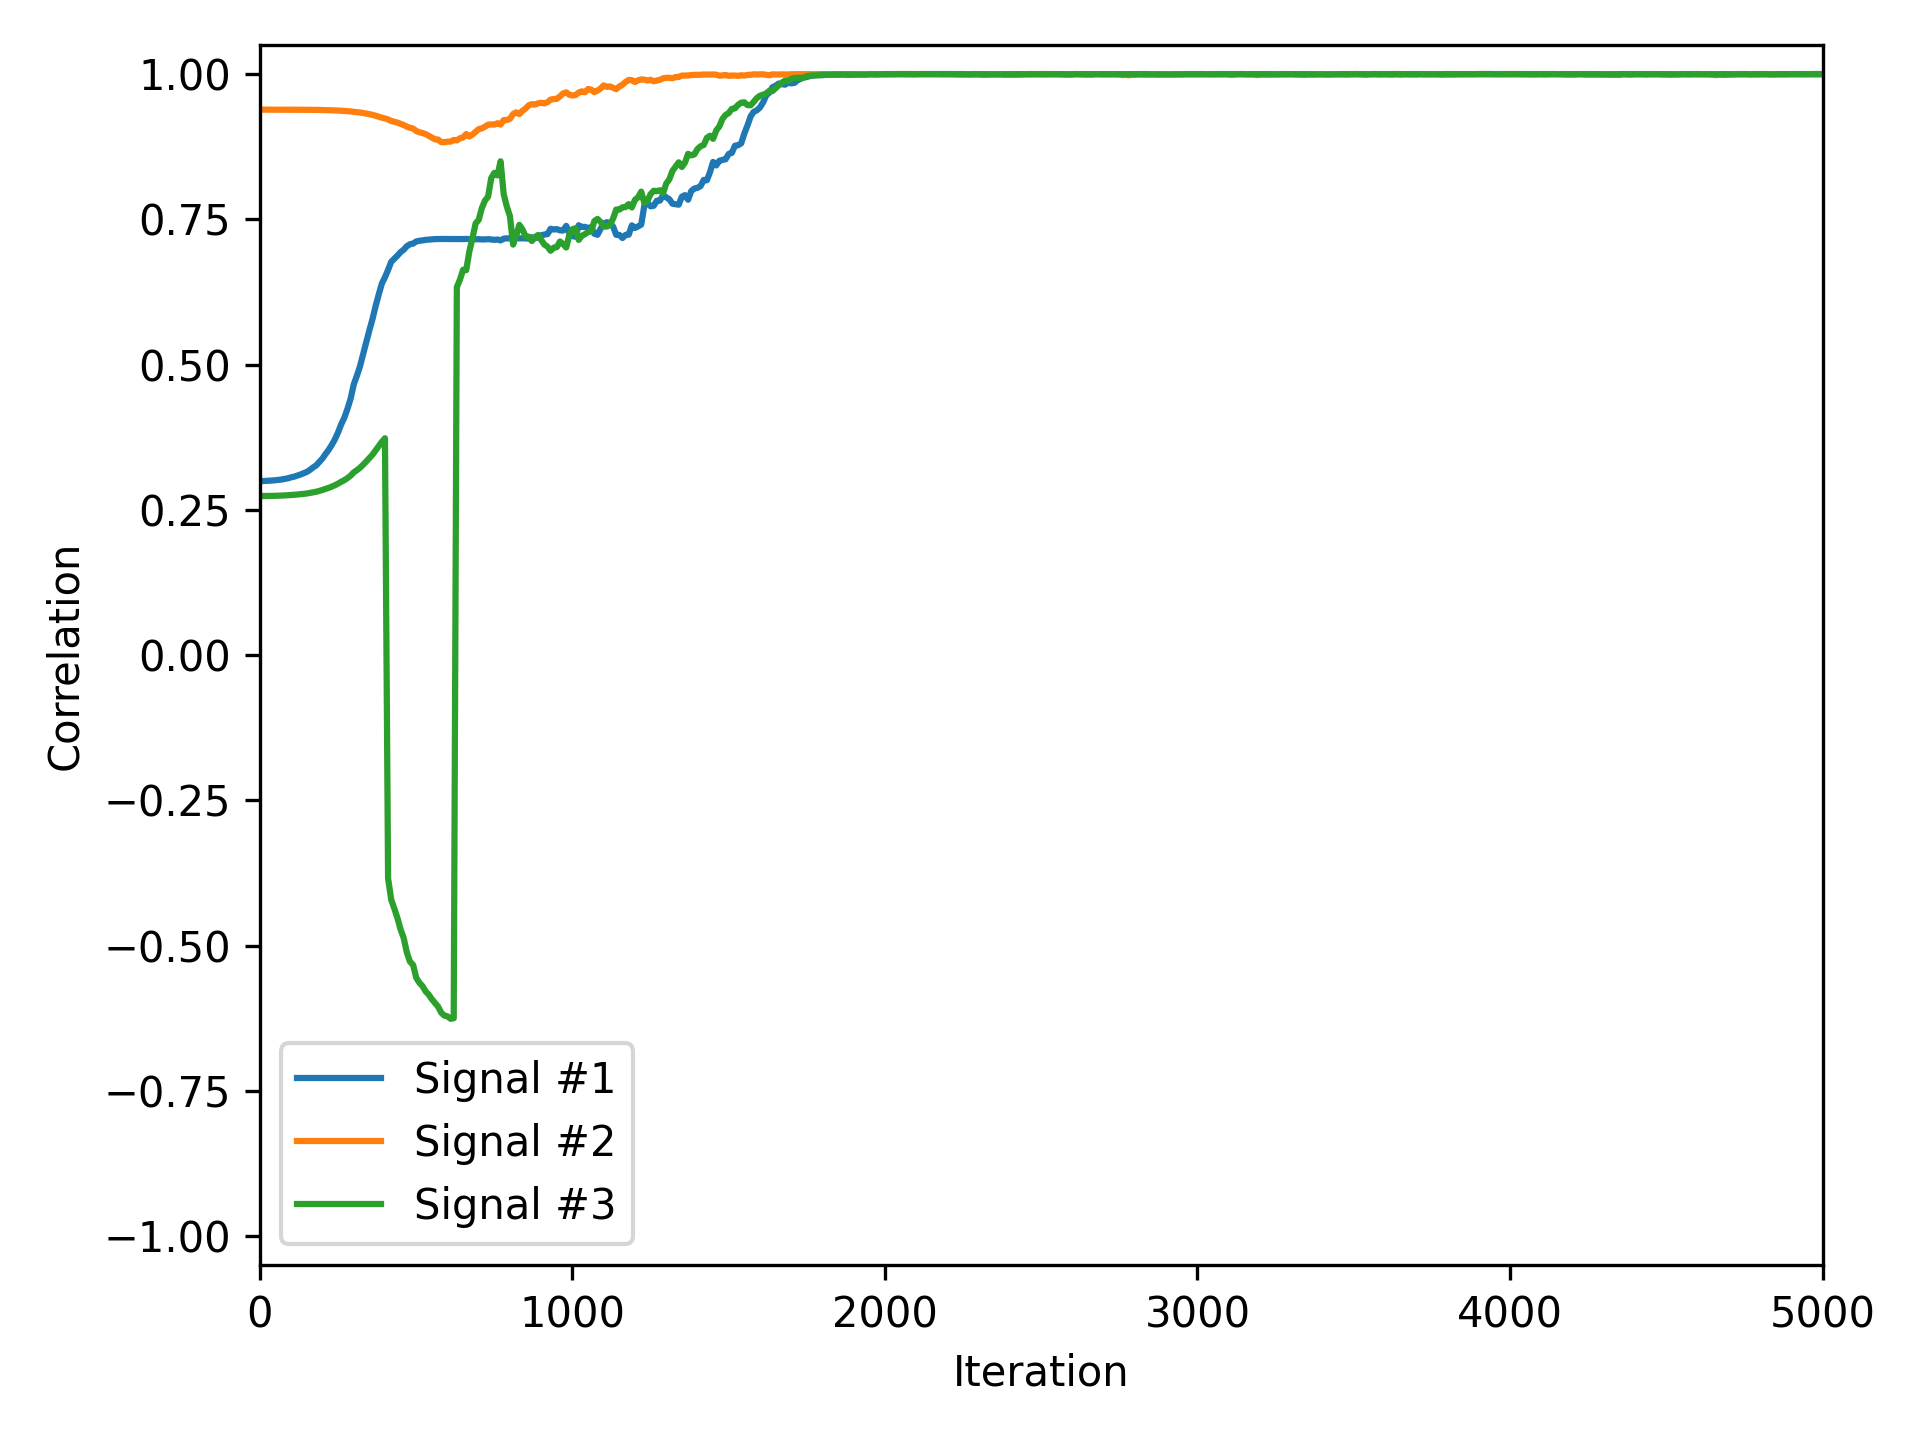
\includegraphics[width=3.6in]{basic_test.png}	
	\caption{Correlation between each source signal and the corresponding the restored signal.}
	\label{fig:basic_test}
\end{figure}

\begin{figure}[!t]
	\centering
	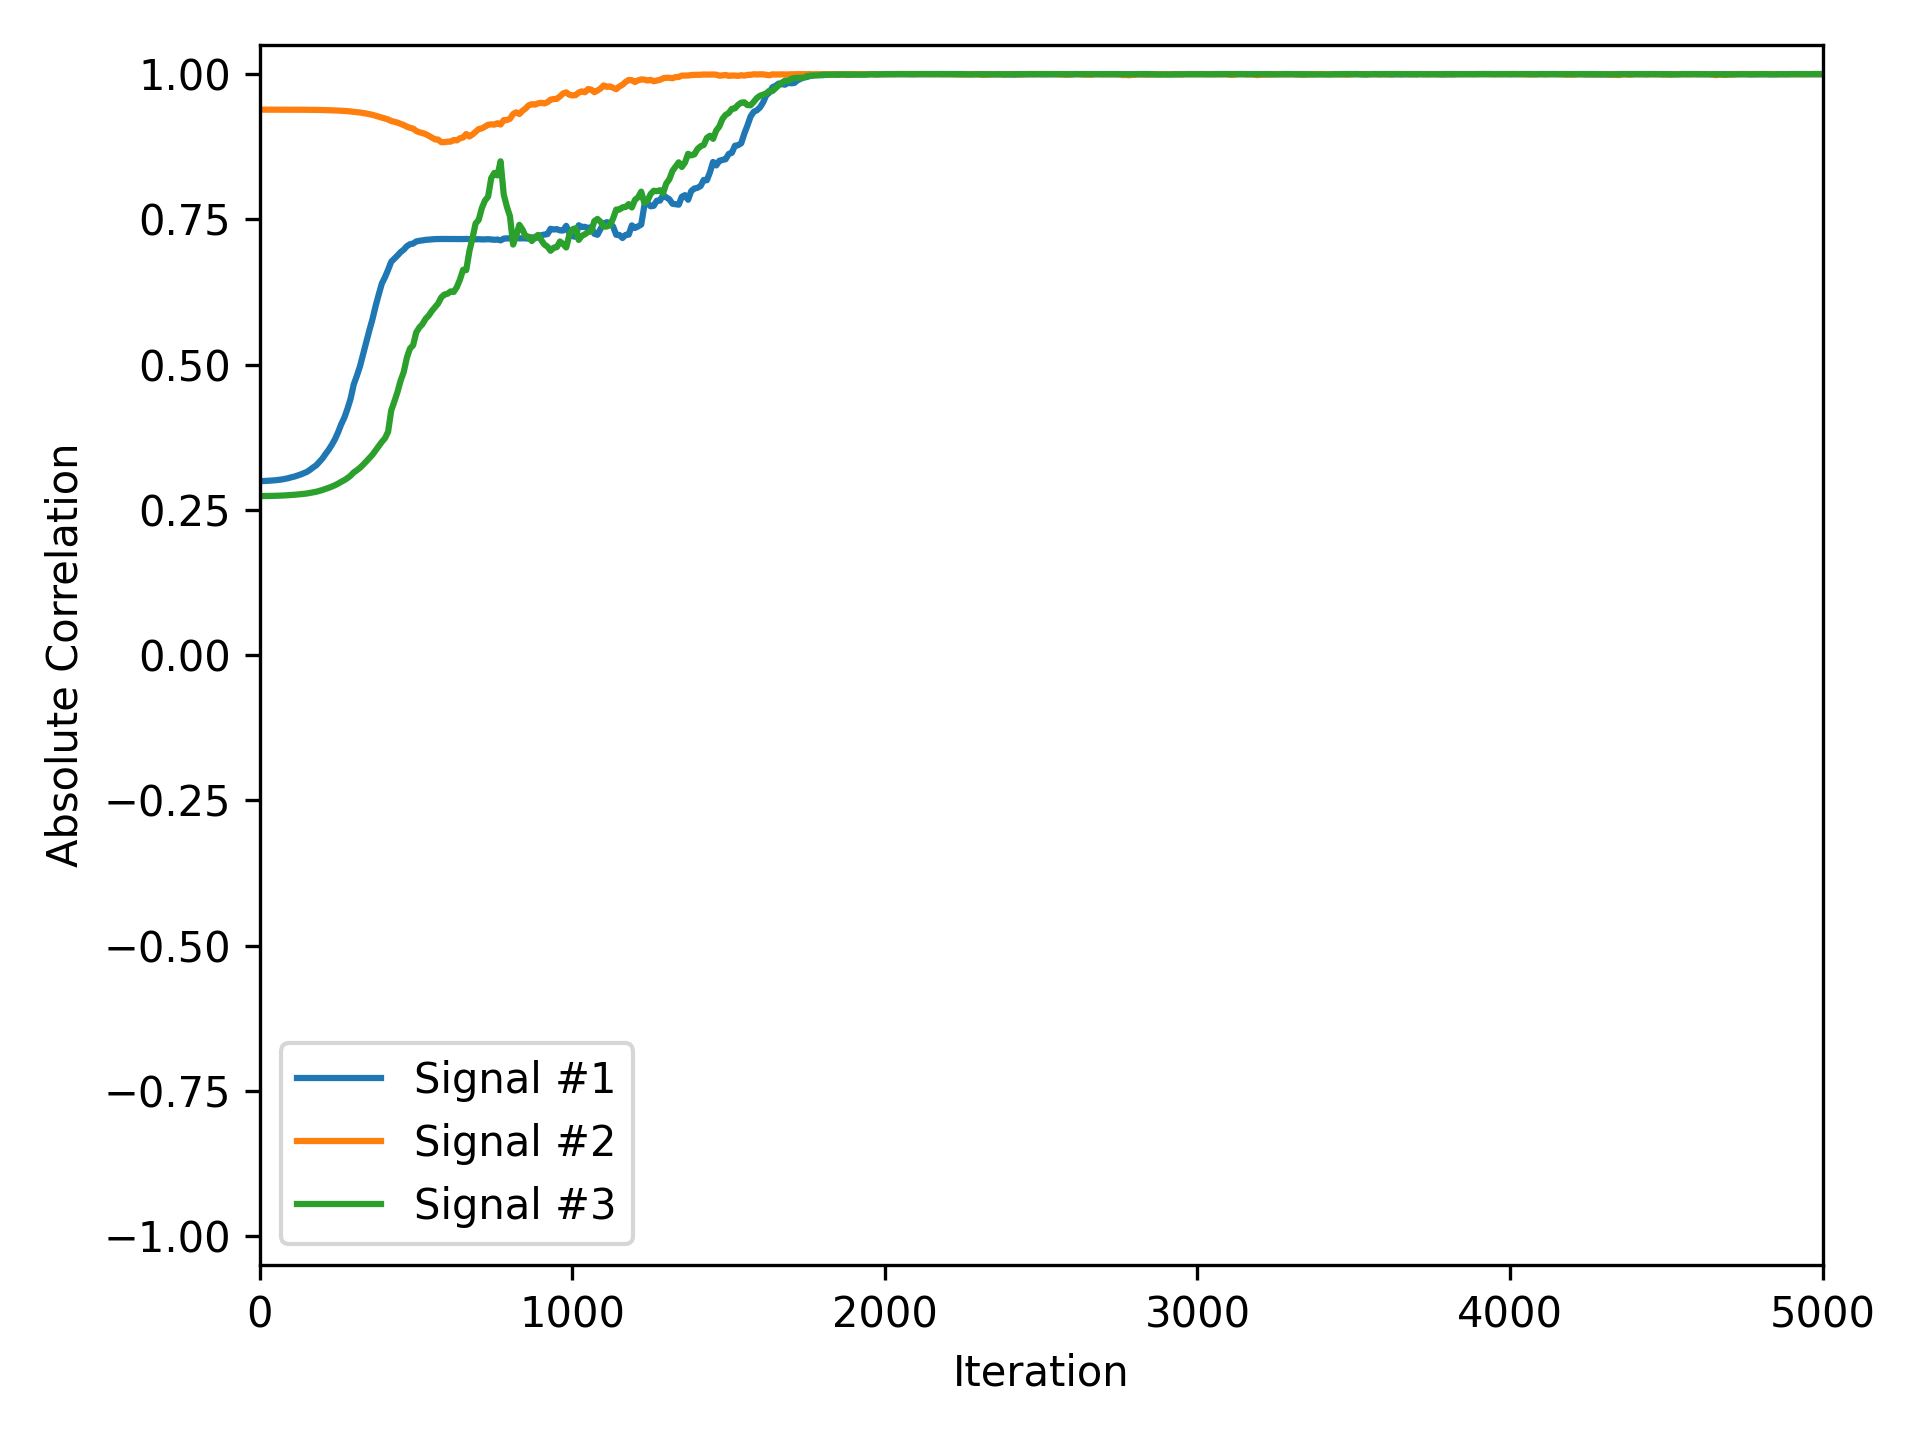
\includegraphics[width=3.6in]{basic_abs_test.png}	
	\caption{Correlation between each source signal and the corresponding the restored signal.}
	\label{fig:basic_abs_test}
\end{figure}

\subsection{Batch size}

The plot of absolute correlation at different batch sizes $t$ is presented in Fig. \ref{fig:batch_abs_test}.
In the experiment, we used $n=3$, $m=3$, $\eta=0.01$, and $k_{\text{max}} = 5000$.
From the results, we can find that the correlation increases fastest at the batch size $k=32$. In a larger batch size, there is a negligible drop at the speed of correlation magnitude increases. On the other hand, a batch size causes a significant drop, which implies that the model suffers from a lack of sample information.

\begin{figure}[!t]
	\centering
	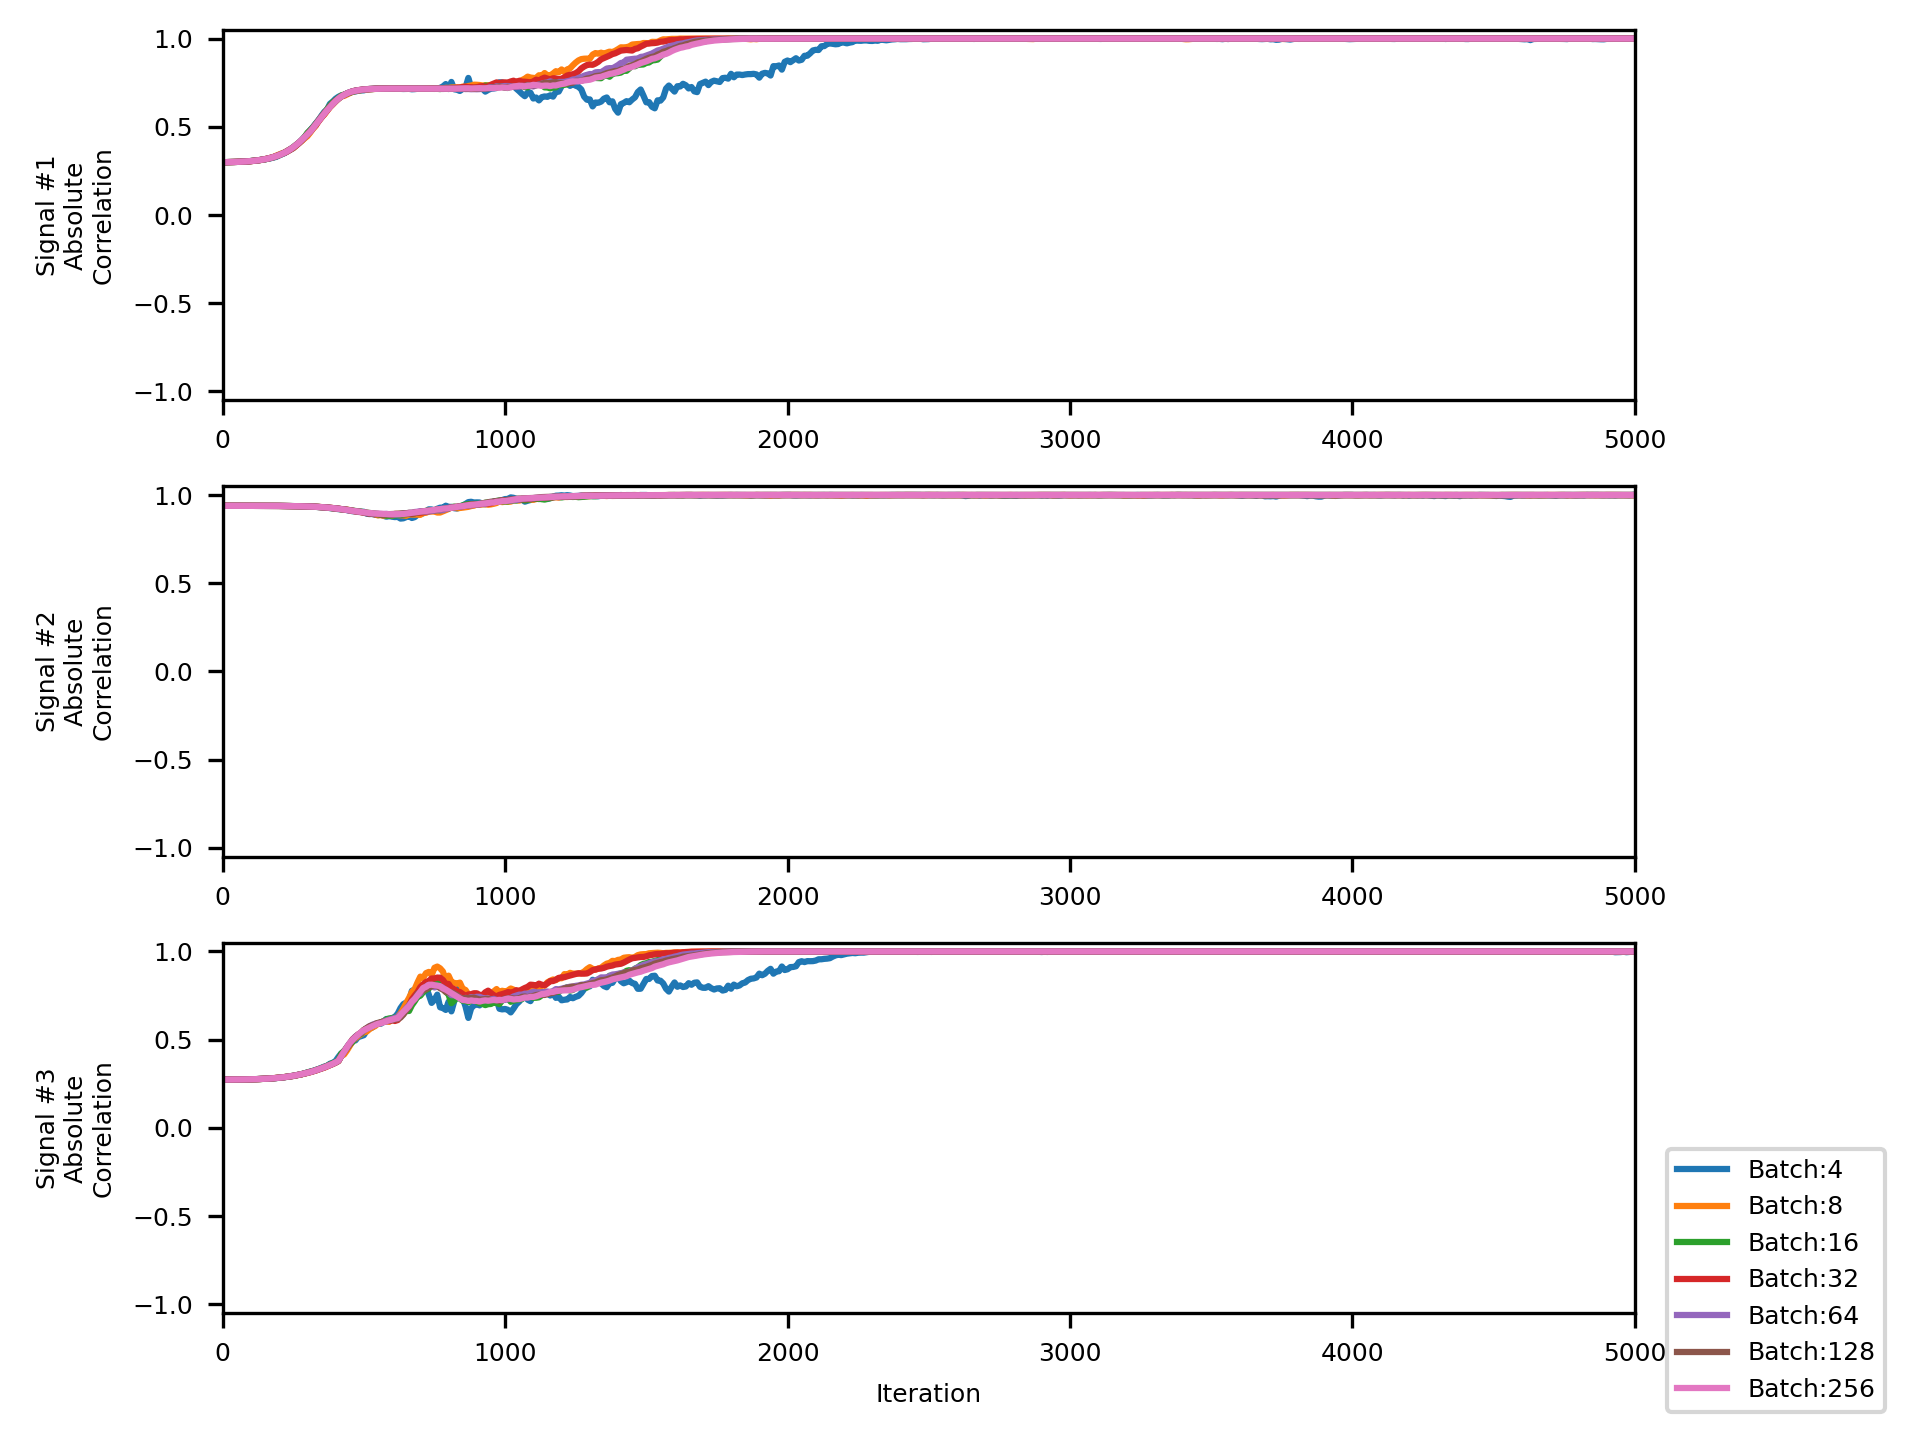
\includegraphics[width=3.6in]{batch_abs_test.png}	
	\caption{Absolute correlation changes on batch size: batch sample sizes are chosen in [4, 8, 16, 32, 64, 128, 256].}
	\label{fig:batch_abs_test}
\end{figure}


\subsection{Learning rate}

The plot of absolute correlation at different learning rates $\eta$ is presented in Fig. \ref{fig:eta_abs_test}.
In the experiment, we used $n=3$, $m=3$, $t=16$, and $k_{\text{max}} = 5000$.
From the results, we can find that a higher learning rate yields faster. However, an excessively high learning rate prevents the convergence at gradient descent, which causes unstable performance, such as perturbations in correlation remaining even after enough iterations.

\begin{figure}[!t]
	\centering
	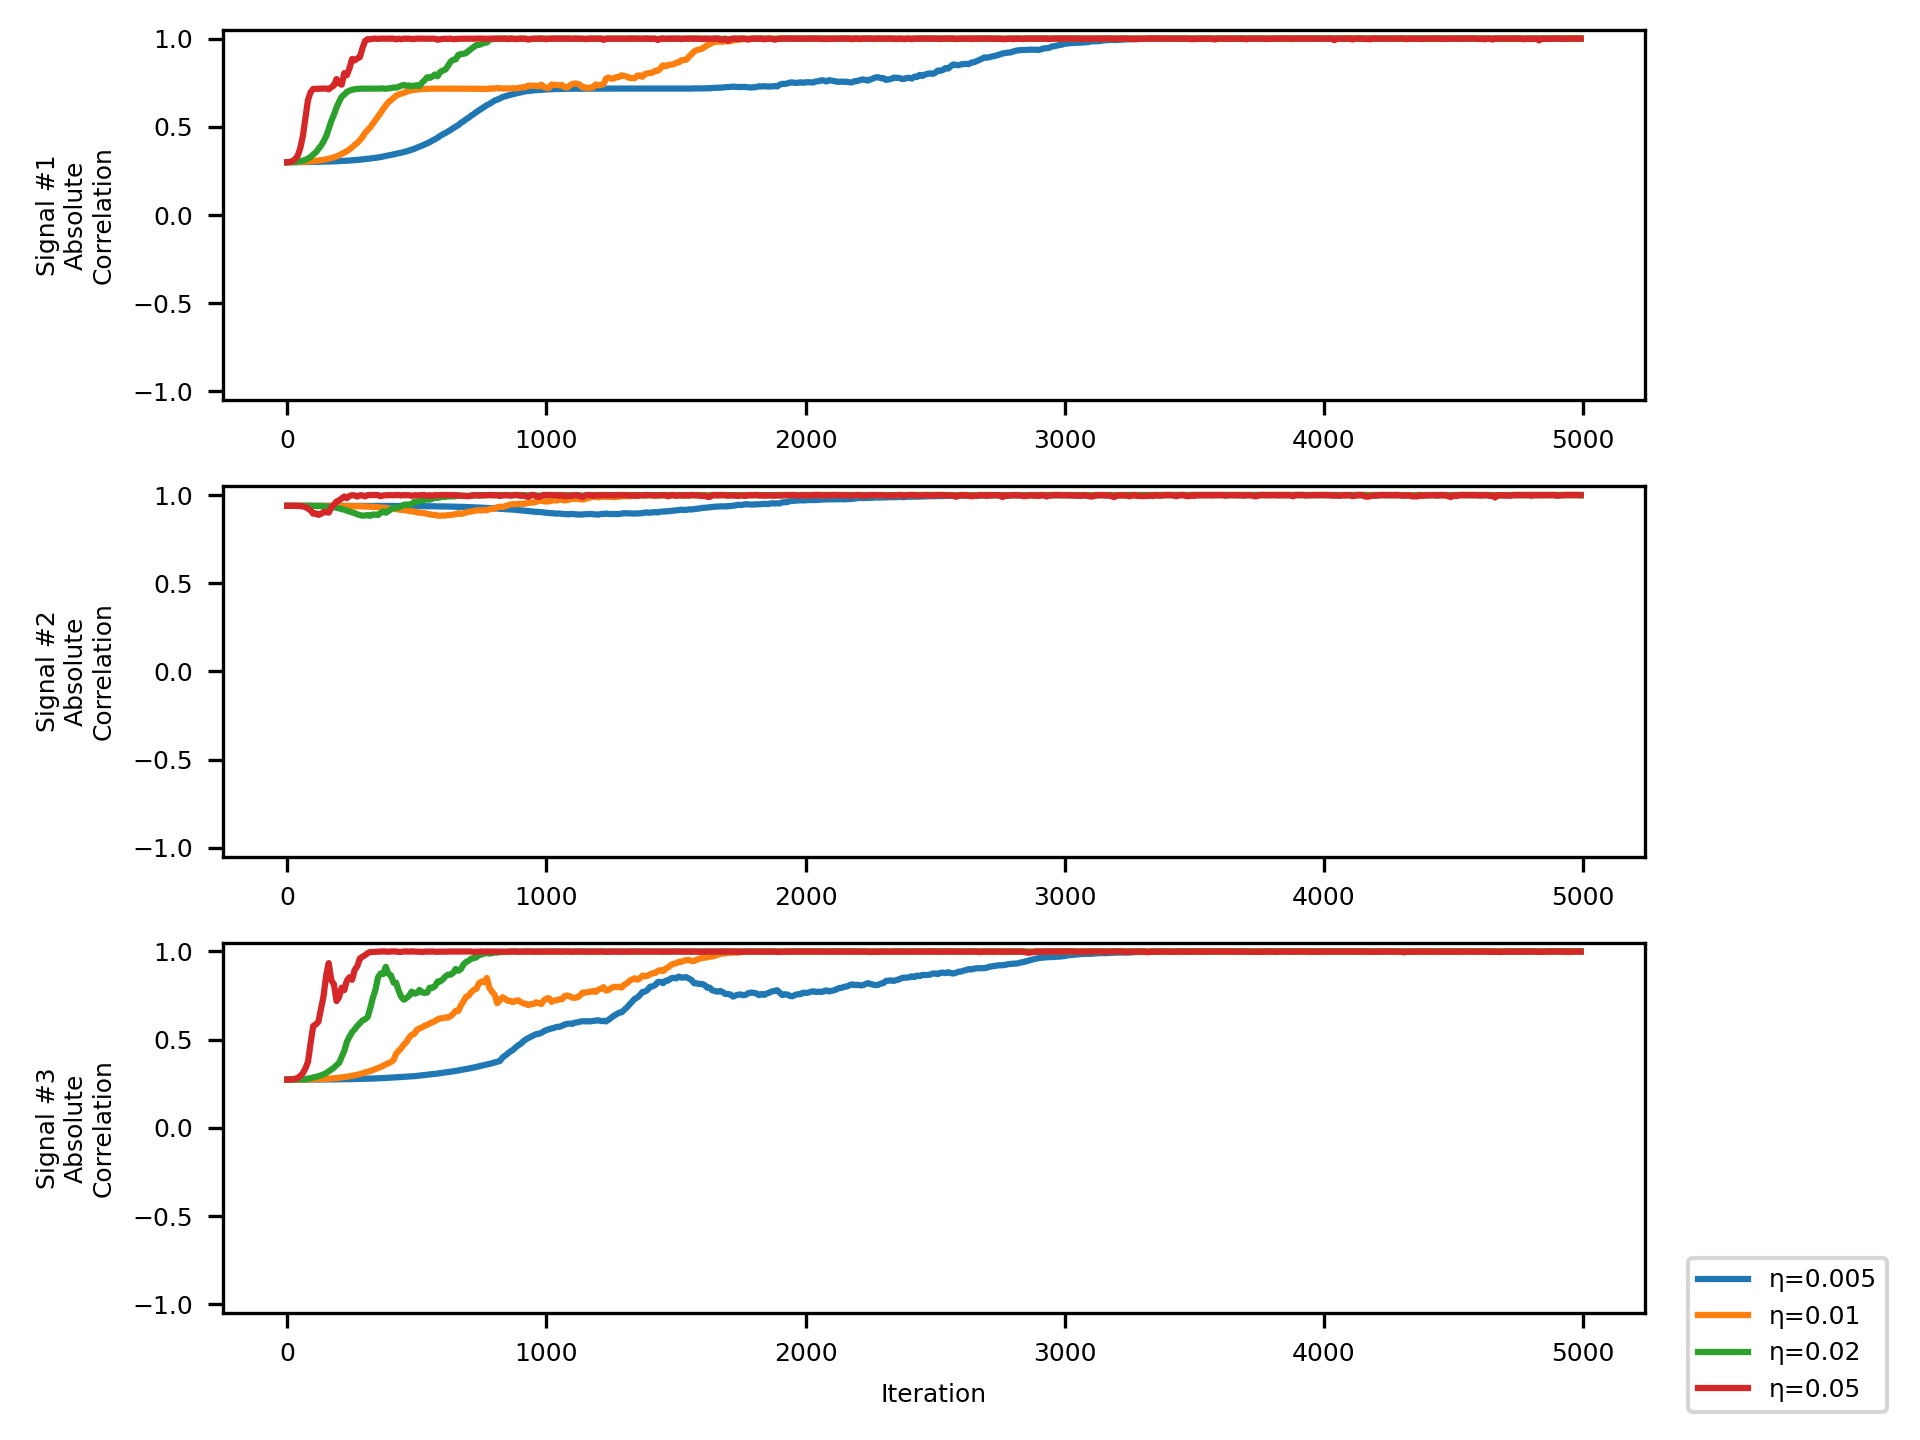
\includegraphics[width=3.6in]{eta_abs_test.png}	
	\caption{Absolute correlation changes on learning rate: learning rates are chosen in [0.005, 0.01, 0.02, 0.05, 0.1, 0.2].}
	\label{fig:eta_abs_test}
\end{figure}



\subsection{Sample size}

The plot of absolute correlation at different sample signal numbers $m$ is presented in Fig. \ref{fig:sample_abs_test}.
In the experiment, we used $n=3$, $t=16$, $\eta=0.01$, and $k_{\text{max}} = 5000$.
From the result at $m=2$, we can find that the model fails to restore Signal \#1. This implies that a smaller sample number than the given source signal number, $m<n$, causes the dimension issue at the unmixing $W$, where the model cannot fully extract the original signals.

\begin{figure}[!t]
	\centering
	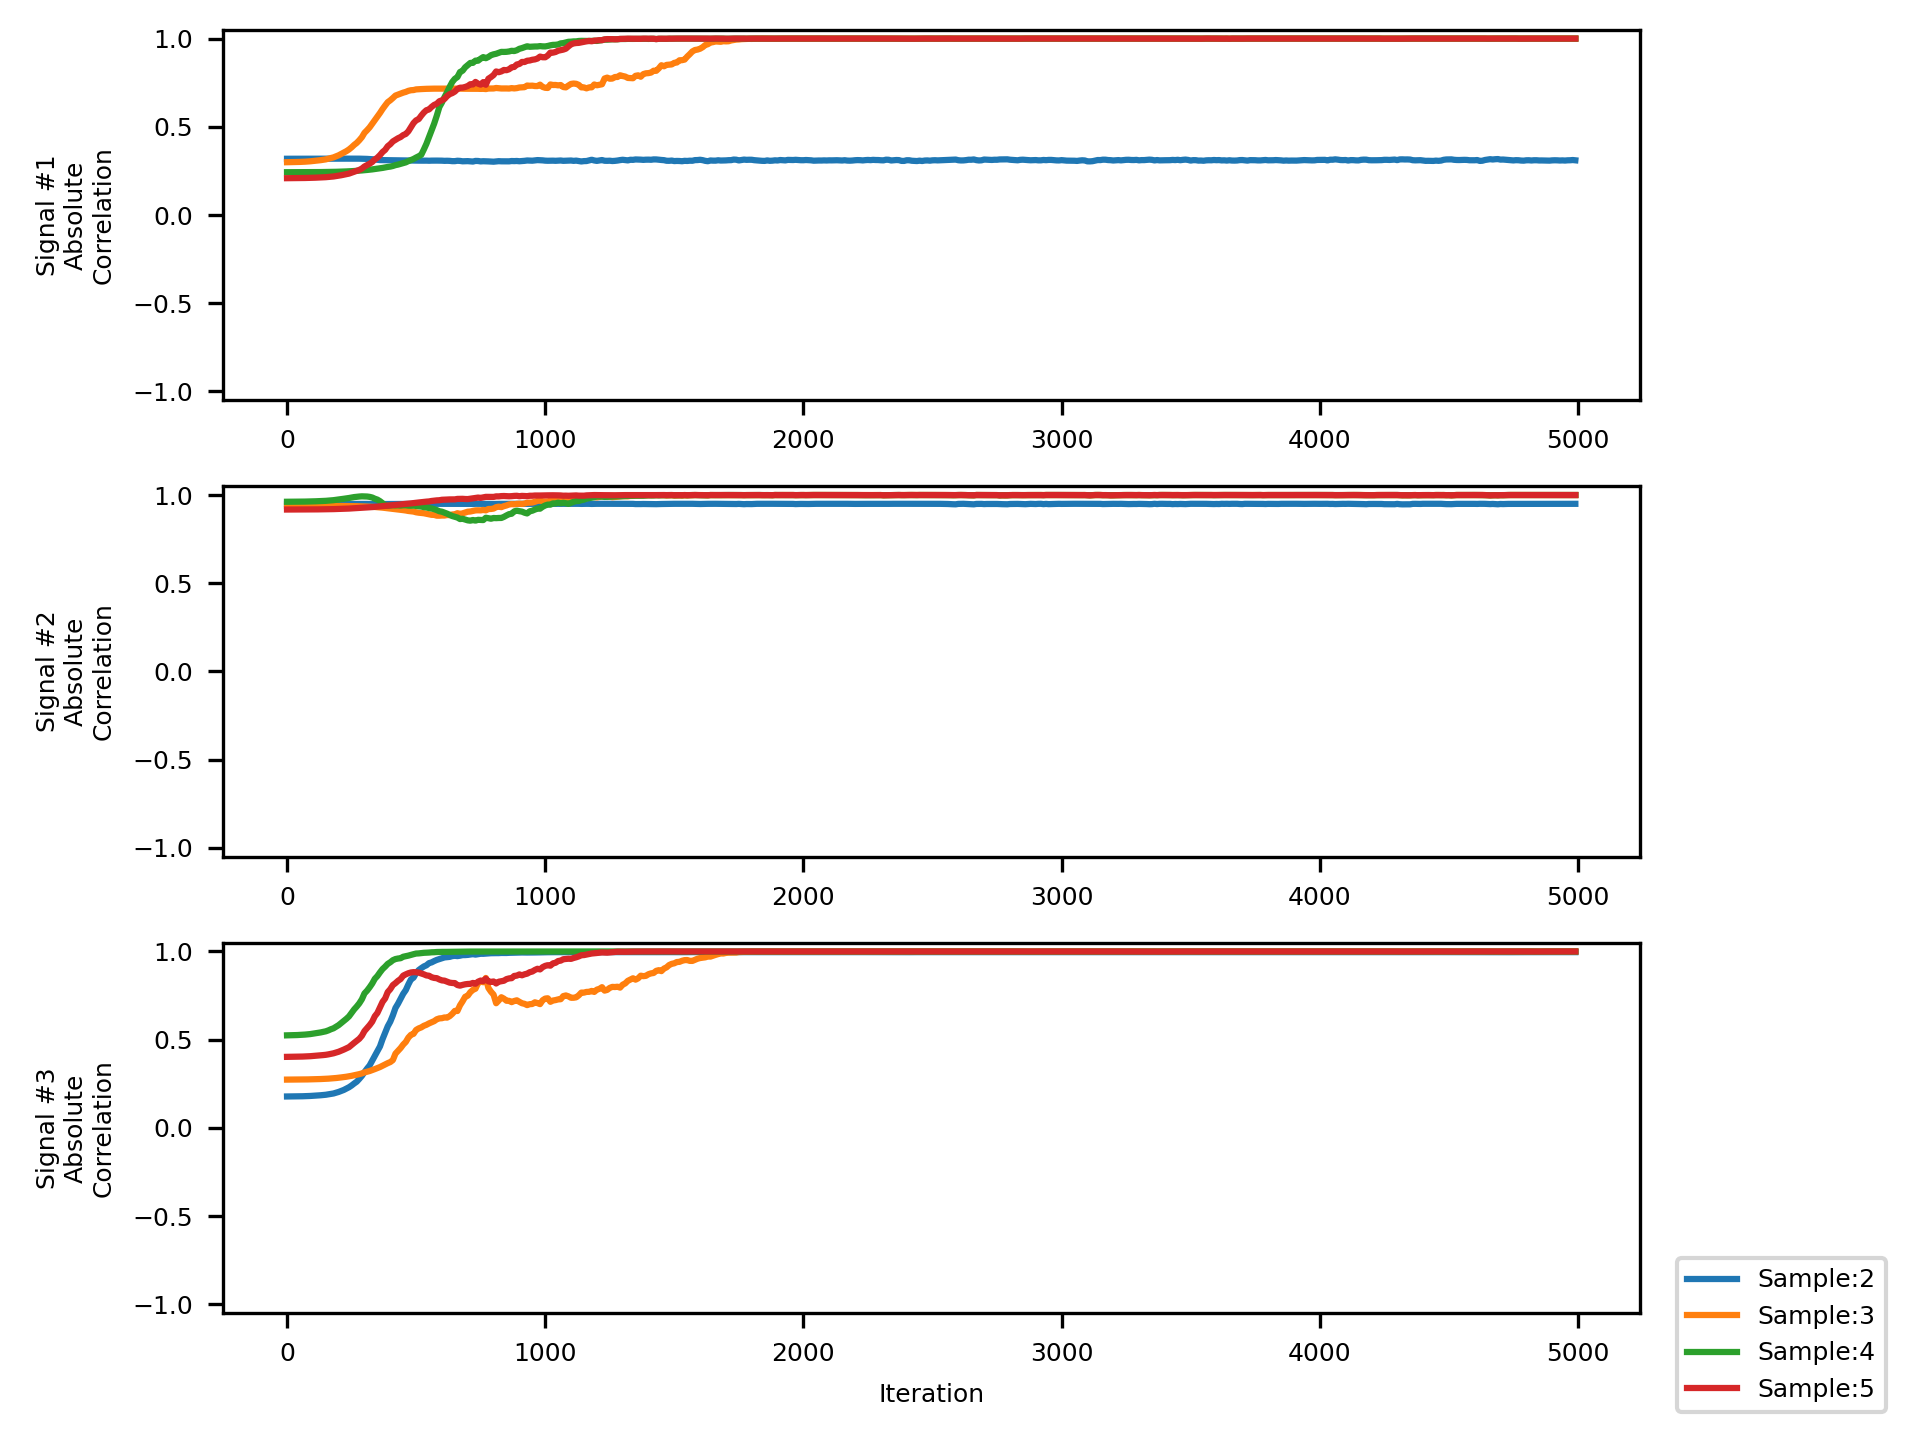
\includegraphics[width=3.6in]{sample_abs_test.png}	
	\caption{Absolute correlation changes on sample sizes: sample sizes are chosen in [2, 3, 4, 5].}
	\label{fig:sample_abs_test}
\end{figure}


\section{Summary} %Intermediate/Preliminary Results: State and evaluate your results upeto the milestone

The ICA method with MLE and gradient descent for separating signals from mixed signals are implemented in the assignment. 
For training, we mixed 5 source sounds of the dataset given at the class webpage and evaluated the model by analyzing the correlation between source signals and restored signals.
From the results of the experiments, we can find the following properties.
First, a small batch size suffers from a slow convergence speed.
Second, there is a trade-off in using a higher learning rate: the convergence speed increases as a learning rate increases but the chance of unstable performance, such as oscillations in correlation, also increases.
Finally, a smaller sample number than a source number fails at full restoration of source signals.
%\section*{Acknowledgments}

%% Use plainnat to work nicely with natbib. 

\bibliographystyle{plainnat}
\bibliography{references}

\end{document}


